\documentclass{beamer}
\usepackage{../common_slides}
\usepackage{tikz}
\usepackage{tikz-qtree}
\usepackage{pdfpages}

\usetikzlibrary{bayesnet}
% \usepackage{enumitem}

\title{Sequence Models 1}
\date{}
\author{CS 287}
\begin{document}

\begin{frame}
  \titlepage
\end{frame}

\begin{frame}{Review: LM Terminology}
  \begin{itemize}
  \item Maximum-likelihood Estimation (MLE)
    \begin{itemize}
    \item Smoothed count-based models are \alert{not} MLE
    \item (Un-regularized) NNLM models \structure{are} MLE
    \item Property of the estimation objective, not the model structure
    \end{itemize}
    \air 

  \item Markov Models
    \begin{itemize}
    \item n-gram models \structure{are} Markov models
    \item windowed NNLM models \structure{are} also Markov models
    \item RNN-LM models are \alert{not} Markovian models
    \item Property of the model structure, not the estimation
    \end{itemize}
  \end{itemize}
\end{frame}

\begin{frame}{Review: Reverse Trie Data structure}


  \begin{center}
    \Tree [ .ROOT [  .mouse($c$) the($c$) ] [  .barks($c$)  [ .dog($c$) the($c$) ] ]  [ .sleeps($c$) [ .dog($c$) the($c$) ] ]  [ .meows($c$) [ .cat($c$) a($c$) ] ]  [ .runs($c$) [ .dog($c$) a($c$) ] [ .cat($c$) the($c$) ]  ] ] ;
  \end{center}

  Used in several standard language modeling toolkits.
\end{frame}


\begin{frame}{Review: RNNs for Language Modeling}
  \begin{itemize}
  \item Recent popularization of RNNs has been based on language modeling (Mikolov, 2012)
    \air

  \item In particular RNNs allow for non-Markovian models
    \[ p(w_i | w_1, \ldots, w_{i-1};\theta) = O(\bolds_i) \]

    \air 

  \item Compare this to the windowed approach.
    \[ p(w_i | w_{i-n+1}, \ldots, w_{i-1};\theta) = O(\bolds_i) \]
  \end{itemize}
\end{frame}

\begin{frame}[allowframebreaks]{Shannon's Markov Babblers}

  \begin{quote}
   
  4. Third-order approximation (trigram structure as in English).

IN NO 1ST LAT WHEY CRATICT FROURE BIRS GROCID
PONDENOME OF DEMONSTURES OF THE REPTAGIN IS
REGOACTIONA OF CRE
  \end{quote}

  \begin{quote}
5. First-Order Word Approximation. Rather than continue with tetragram,
... , II-gram structure it is easier and better to jump at this
point to word units. Here words are chosen independently but with
their appropriate frequencies.

REPRESENTING AND SPEEDILY IS AN GOOD APT OR
COME CAN DIFFERENT NATURAL HERE HE THE A IN
CAME THE TO OF TO EXPERT GRAY COME TO FURNISHES
THE LINE MESSAGE HAD BE THESE.

  \end{quote}

  \begin{quote}
    6. Second-Order Word Approximation. The word transition probabilities
are correct but no further structure is included.

THE HEAD AND IN FRONTAL ATTACK ON AN ENGLISH
'RITER THAT THE CHARACTER OF THIS POINT IS
THEREFORE ANOTHER METHOD FOR THE LETTERS
THAT THE TIME OF WHO EVER TOLD THE PROBLEM
FOR AN UNEXPECTED

The resemblance to ordinary English text increases quite noticeably at
each of the above steps.

  \end{quote}
\end{frame}


\begin{frame}{Non-Markov Babblers}
  \begin{itemize}
  \item Use previous prediction $\hat{\boldy}$ to decide on next word.
    \air

  \item In particular RNNs allow for non-Markovian models
    \[ p(w_i | w_1, \ldots, w_{i-1};\theta) = \hat{\boldy_i} =  O(\bolds_i) \]

    \air 

  \item Greedy non-Markov babbler:
    \[ w_{i+1} = \argmax_{w} \hat{y}_{i,w} \]
  \end{itemize}
\end{frame}


\begin{frame}{Babbling Visually}
  \begin{center}
  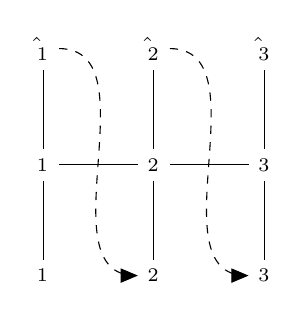
\begin{tikzpicture}
    \node(ya){$\hat{\boldy}_1$}; 

    \node(sa)[below=of ya]{$\bolds_1$}; 
    \node(xa)[below=of sa]{$\boldx_1$}; 
    \node(yb)[right=of ya]{$\hat{\boldy}_2$}; 
    \node(sb)[below=of yb]{$\bolds_2$}; 
    \node(xb)[below=of sb]{$\boldx_2$}; 
    \node(yc)[right=of yb]{$\hat{\boldy}_3$}; 
    \node(sc)[below=of yc]{$\bolds_3$}; 
    \node(xc)[below=of sc]{$\boldx_3$}; 
    \draw (sa) edge (sb); 
    \draw (sb) edge (sc); 


    \draw (sa) -- (xa); 
    \draw (sb) -- (xb); 
    \draw (sc) -- (xc); 
    \draw (sa) -- (ya); 
    \draw (sb) -- (yb); 
    \draw (sc) -- (yc); 

    \draw (ya) edge[dashed, out=0,in=180,->] (xb); 
    \draw (yb) edge[dashed, out=0,in=180,->] (xc); 
  \end{tikzpicture}
  \end{center}
\end{frame}

\begin{frame}{Diversity in Babbling}
  \begin{itemize}
  \item Taking the greedy solution can lead to boring output.
    \air 

  \item Instead can  sample from soft-max distribution,
    \[  \hat{\boldy} \sim \softmax(\bolds_i \boldW + \boldb)\]
    \air 

  \item However this can lead to non-fluent output.
  \end{itemize}

\end{frame}

\begin{frame}{Review: Why is it called the softmax?}

  \begin{columns}[t]
    \begin{column}[t]{0.5\textwidth}


      \begin{figure}
        \centering
        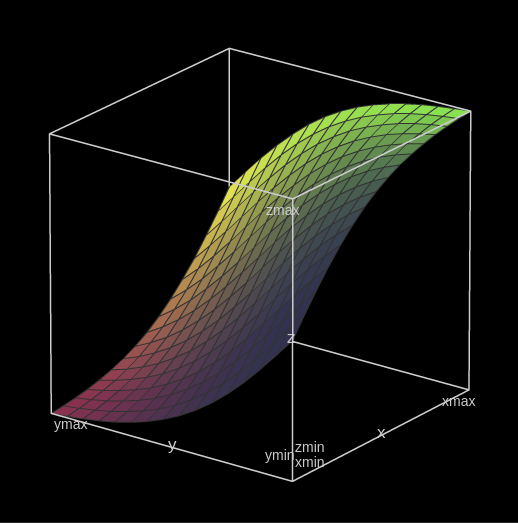
\includegraphics[width=5cm]{softmax}
      \end{figure}
      \[\softmax([x\ y]) = \frac{\exp(x)}{\displaystyle  \exp(x) + \exp(y)}  \]
    \end{column}

    \begin{column}[t]{0.5\textwidth}


      \begin{figure}
        \centering
      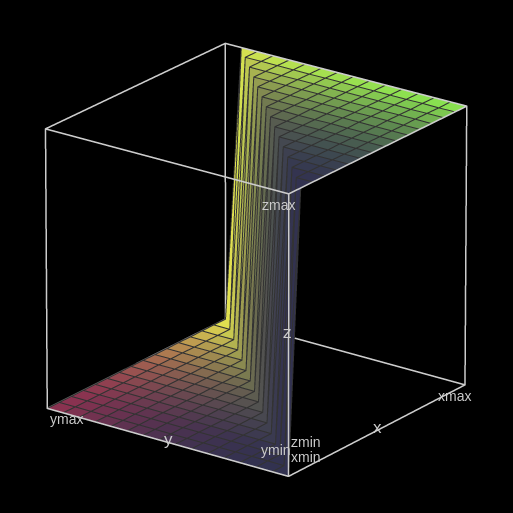
\includegraphics[width=5cm]{argmax}
      \end{figure}
      \[\argmax([x\ y]) = \indicator(x > y) \]
    \end{column}
  \end{columns}
\end{frame}


\begin{frame}{Temperature}
  \begin{itemize}
  \item Can use a temperature parameter $t \in (0, 1]$ to modulate

    \air
  \item Temperature-based sampling.
      \[\hat{\boldy} \sim \softmax((\bolds_i \boldW + \boldb)/t)\]

      \air
      
    \item What happens when the parameter is closer to the extremes?
  \end{itemize}
\end{frame}

\begin{frame}{Temperature $t=0.99$}
  \begin{center}
    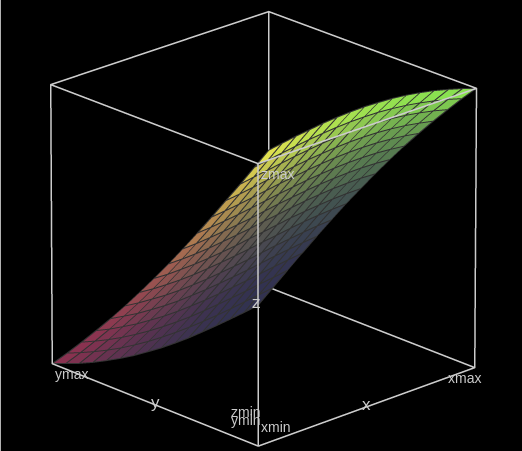
\includegraphics[width=0.8\textwidth]{sm99}
  \end{center}
\end{frame}
\begin{frame}{Temperature $t=0.5$}
  \begin{center}
    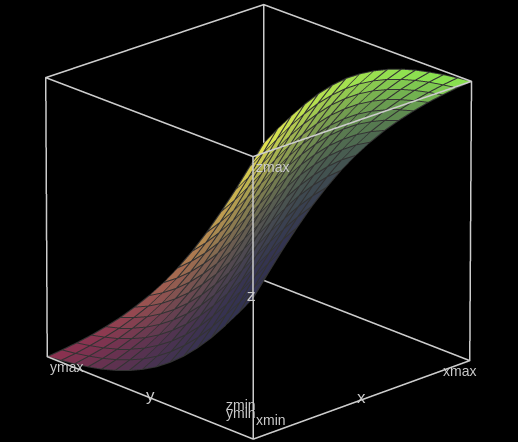
\includegraphics[width=0.8\textwidth]{sm5}
  \end{center}
\end{frame}

\begin{frame}{Temperature $t=0.01$}
  \begin{center}
    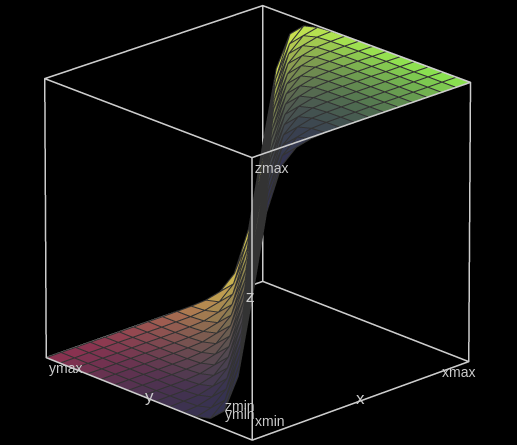
\includegraphics[width=0.8\textwidth]{sm01}
  \end{center}
\end{frame}

\begin{frame}{Temperature $t=0.001$}
  \begin{center}
    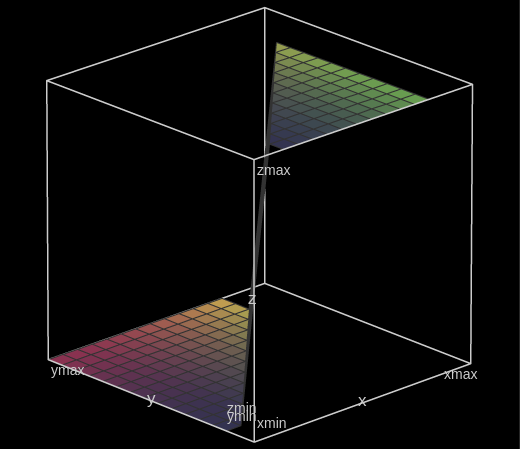
\includegraphics[width=0.8\textwidth]{sm001}
  \end{center}
\end{frame}


\begin{frame}{Quiz: Babbling for Segmentation}
  The upcoming homework asks you to insert spaces in a 
  non-segmented stream of characters using an RNN transducer.
  For example given

  \begin{center}
    \texttt{t h e d o g w a l k s t o t h e p a r k}
  \end{center}

  You should output,

  \begin{center}
    \texttt{the dog walks to the park}.
  \end{center}
  
  How might you do this efficiently with a RNN transducer?  What does
  the training look like and how do you generate the output with a
  greedy babbler?
\end{frame}

\section{Sequence Models}

\begin{frame}
  
\end{frame}

\begin{frame}
  
\end{frame}

\begin{frame}{So Far: Multiclass Classification}
  Every problem:
  \begin{itemize}
  \item Input encoding $\boldx$ (sparse or dense)
    \air 

  \item Output encoding $\boldy$ (sparse index $\mcC$)
    \air 
  
  \item Prediction $\hat{\boldy}$  
    \air 
    
  \item Classification 
    \[c = \argmax_{i\in \mcC} y_i \]
  \end{itemize}
\end{frame}

\begin{frame}{Predicting Structure}
  What if we want to predict:
  \begin{itemize}
  \item Parse trees
    \air 

  \item Named-entities
    \air 

  \item Semantic Roles
  \end{itemize}
\end{frame}

\begin{frame}{Example: BIO Tagging}
  \begin{description} \itemsep 20pt
  \item[B-TYPE] Stop current mention and begin new mention
    \air 
  \item[I-TYPE] Continue adding to current mention
  \item[O ] Not part of a mention.
  \end{description}
  \pause
  
  \textbf{Example:} \air

  \texttt{[PER \alert{George Bush} ]  [LOC \structure{U.S.} ] president is traveling to [LOC \alert{Baghdad} ] .  } 
\end{frame}

\begin{frame}{Better Tag Features: Tag Sequence}
  Representation can use specific aspects of text.
  \begin{itemize}
  \item $\mcF$; Prefixes, suffixes, hyphens, first capital, all-capital, hasdigits, etc.
  \item \structure{Also} include features on previous tags
  \end{itemize}

  Example: Rare word tagging with context

  \begin{center}
    \texttt{in \structure{130/CD} \alert{regular-season/*} games ,}
  \end{center}
  \begin{eqnarray*}
    \boldx &=& \delta(\texttt{last:CD}) + \delta(\texttt{prefix:3:reg}) + \delta(\texttt{prefix:2:re}) \\
    &+& \delta(\texttt{prefix:1:r}) + \delta(\texttt{has-hyphen}) \\
    &+& \delta(\texttt{lower-case}) + \delta(\texttt{suffix:3:son}) \ldots
  \end{eqnarray*}
\end{frame}



\begin{frame}{Standard Approach}
  
  
  \[ \hat{\boldy} = \softmax( \boldx \boldW + \boldb)  \] 
  \begin{itemize}
  \item Let $\mcC$ to all possible tag sequences.
    \air 
  \item Let $\boldx$ to be a representation of whole sentence.
    \air 
  \item Let $\hat{\boldy}$ be distribution over tag sequences.
    \air 

  \item What breaks down? 
  \end{itemize}
\end{frame}

\begin{frame}{Issues with Multiclass for Sequences }
  \begin{itemize}
  \item Say there are $\mcT$ tags and sequence length is $n$
    \air 

  \item There are $\dout = O(\mcT^n)$ sequences! 
    \air 
  \item Just naively computing the softmax is exponential in length. 
    \air 

  \item Even if you could compute the softmax, $\boldW \in \reals^{\din \times \dout}$ would 
    be impossible to train.
  \end{itemize}
\end{frame}

\begin{frame}{Predicting Structure}
  Instead we will try to maximize over the sequence,
  \[ \argmax_{c_1 \in \mcC, \ldots, c_n\in \mcC} f(\boldx, c_1, \ldots, c_n; \theta)\]
\end{frame}


\begin{frame}{What is the function $f$}
  \begin{itemize}
  \item Allow many different functions.
  \end{itemize}
\end{frame}

\begin{frame}{Encoding Output}
  We will assume that,
  \begin{itemize}
  \item Assume true output is a sequence,
    \[ \boldy_1, \ldots \boldy_n\] 
    \air
  \item Each is a sparse one-hot vector
  \end{itemize}
\end{frame}

\section{Hidden Markov Model}

\begin{frame}{Hidden Markov Model}
  \begin{itemize}
  \item Natural extension of naive Bayes to sequences.
    \air 
  \item Allows us to efficiently solve argmax,
    \[ \argmax_{\hat{\boldy} \in \mcY} f(\boldx, \hat{\boldy}; \theta)\]
  \end{itemize}
\end{frame}

\begin{frame}{Review: Multinomial Naive Bayes } 
  % Estimate 
  Reminder, joint probability chain rule,  

  \[ p(\boldx, \boldy) = p(\boldx | \boldy) p(\boldy) \] 


    \pause
  For a sparse features, with observed classes we can write as,
  
  \begin{eqnarray*}
    p(\boldx, \boldy) &=& p(x_{f_1}=1, \ldots, x_{f_k}=1 | \boldy=\bolddelta(c) ) p(\boldy=\bolddelta(c)) =\\
     &=& \prod_{i=1}^k p(x_{f_i}=1 | x_{f_1}=1, \ldots, x_{f_{i-1}}=1, \boldy=\bolddelta(c)) p(\boldy=\bolddelta(c)) \approx \\
     &=& \prod_{i=1}^k p(x_{f_i} =1| \boldy) p(\boldy)  
  \end{eqnarray*}

  
  First is by chain-rule, second is by independence assumption.
\end{frame}


\begin{frame}{Naive Bayes}
  Graphical model representation,
  \begin{center}
    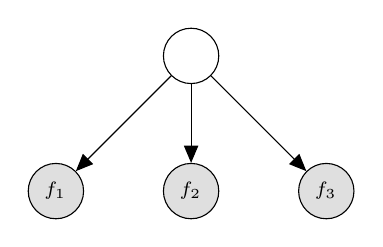
\begin{tikzpicture}
      % Define nodes
      \node[obs] (xa) {$\boldx_{f_1}$}; \node[obs, right=of xa] (xb)
      {$\boldx_{f_2}$}; \node[obs, right=of xb] (xc) {$\boldx_{f_3}$};
      \node[latent, above=of xb] (y) {$\boldy$};
    
      % Connect the nodes
      \edge {y} {xa, xb, xc} ; %
    \end{tikzpicture}
  \end{center}
  For simplicity,  assume that there is only one space feature in $x$.
\end{frame}



\begin{frame}{Generative Sequence Model}
  \begin{itemize}
  \item Define the function $f$ to be the joint probability,

  \[ f(\boldx, c_1, \ldots, c_n) = p(\boldy_1=\delta(c_1), \ldots, \boldy_n=\delta(c_n), \boldx_1, \ldots, \boldx_n) \] 

  \air 

  \item Aim will be to maximize this,
    \[ \argmax_{c_1 \in \mcC, \ldots, c_n\in \mcC} f(\boldx, c_1, \ldots, c_n; \theta)\]
  \end{itemize}

  \begin{eqnarray*}
  
  \end{eqnarray*}
  
\end{frame}

\begin{frame}{Hidden Markov Model}
  \begin{eqnarray*}
    f(\boldx, c_1, \ldots, c_n; \theta) &=& \\ p(\boldy_1=\delta(c_1), \ldots, \boldy_n=\delta(c_n), \boldx_1, \ldots, \boldx_n)  \\
    &=& \prod_{i=1}^n p(\boldx_i | \boldx_1, \ldots \boldx_{i-1}, \boldy_1, \ldots, \boldy_n) p(\boldy_i=\delta(c_i) | \boldy_1=\delta(c_1) \ldots \boldy_{i-1}=\delta(c_{i-1})) \\
    &\approx& \prod_{i=1}^n p(\boldx_i | \boldy_i = \delta(c_i)) p(\boldy_i=\delta(c_i) | \boldy_{i-1}=\delta(c_{i-1}), \boldx_1, \ldots, \boldx_n) \\
    &\approx& \prod_{i=1}^n p(\boldx_i | \boldy_i = \delta(c_i)) p(\boldy_i=\delta(c_i) | \boldy_{i-1}=\delta(c_{i-1})) \\
  \end{eqnarray*}
\end{frame}

\begin{frame}{Example: Hidden Markov Model}
\begin{center}  
  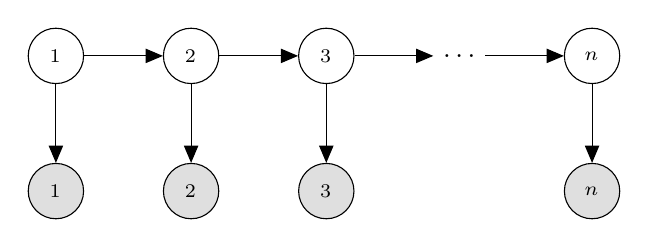
\begin{tikzpicture}
    \node (Ea) [obs] {$\boldx_1$}; 
    \node (Xa) [latent,above =of Ea] {$\boldy_1$}; 

    \node (Eb) [obs, right = of Ea ] {$\boldx_2$}; 
    \node (Xb) [latent,above =of Eb] {$\boldy_2$}; 

    \node (Ec) [obs, right = of Eb] {$\boldx_3$}; 
    \node (Xc) [latent,above =of Ec] {$\boldy_3$}; 
    \node (Xd) [right =of Xc] {$\ldots$}; 
    \node (Xe) [latent,right =of Xd] {$\boldy_n$}; 
    \node (Ee) [obs,below =of Xe] {$\boldx_n$}; 

    \edge {Xa} {Xb} ; %
    \edge {Xb} {Xc} ; %
    \edge {Xa} {Ea} ; %
    \edge {Xb} {Eb} ; %
    \edge {Xc} {Ec} ; %
    \edge {Xc} {Xd} ; %
    \edge {Xd} {Xe} ; %
    \edge {Xe} {Ee} ; %
  \end{tikzpicture}
\end{center}  
\end{frame}


\begin{frame}{Hidden Markov Model}
  Hidden Markov model requires two distributions,
  \begin{itemize}
  \item Transition distribution 
    \[p(\boldy_i | \boldy_{i-1}; \theta)\]
  \item Emission distribution
    \[ p(\boldx_i | \boldy_i ; \theta)\] 
  \end{itemize}


  \begin{itemize}
  \item How many total parameters?
  \end{itemize}
\end{frame}

\begin{frame}{Multinomial Hidden Markov Model}
  (Should look familiar)
  \begin{itemize}
  \item  Both  $p(\boldy_i | \boldy_{i=1})$ and $p(\boldx_i | \boldy_i)$ are
    parameterized as multinomials.
    
  \item Fit first using count matrix $\boldT$,
    \begin{itemize}
      \item Let $T_{c',c}$ be the counts of class $c'$ preceding class $c$.

      \item \[p(\boldy_i = \bolddelta(c_i) | \boldy_{i-1} = \bolddelta(c_{i-1})) = \frac{T_{c', c}}{T_{\cdot,c}} \]
    \end{itemize}
    \pause

  \item Fit second using count matrix $\boldF$ ,
    \begin{itemize}
      \item Let $F_{f,c}$ be the counts of emission $f$ with class $c$.
      \item Then,
      \[p(\boldx_i=\bolddelta(f) | \boldy_i=\bolddelta(c)) = \frac{F_{f, c}}{F_{\cdot,c}}  \]     
    \end{itemize}
  \end{itemize}
\end{frame}



\begin{frame}{Example: Named-Entity Recognition}  
\begin{verbatim}
   U.N.         NNP  I-NP  I-ORG 
   official     NN   I-NP  O 
   Ekeus        NNP  I-NP  I-PER 
   heads        VBZ  I-VP  O 
   for          IN   I-PP  O 
   Baghdad      NNP  I-NP  I-LOC 
   .            .    O     O 
\end{verbatim}


  \begin{itemize}
  \item $F$ is constructed by counting up rows
    \air 
  \item $T$ is constructed by iterating over column
    \air
  \item Standard multinomial MLE issues apply (smoothing, rare-words)
    air 
  \item Can extend $F$ to multiple features as in naive Bayes 
  \end{itemize}
\end{frame}

\begin{frame}{Versus Multiclass}
  Exercise: How does this model improve upon previous setup?
  \begin{itemize}
  \item Number Parameters?
    \air 
  \item Producing a solution?
    \air 

  \item Types of features?
  \end{itemize}
\end{frame}

\section{Maximum-Entropy Markov Models}

\begin{frame}{Discriminative Sequence Models}
  \begin{itemize}
  \item Just as with multiclass, we can instead fit the conditional probability.
    \air 

  \end{itemize}
\end{frame}

\begin{frame}{Review: Multiclass Logistic Regression}
  \begin{itemize}
  \item Direct estimation of conditional $p(\boldy =c | \boldx; \theta)$

    \[\hat{\boldy} =  p(\boldy =c | \boldx; \theta) =  \softmax(\boldx \boldW + \boldb) \]
  \item $\boldW \in \reals^{\din \times \dout}, \boldb \in \reals^{1 \times \dout}$; model parameters

  \item ``Regression'' of the distribution.
  \item Classification still done as,
    \[ \hat{c} =  \argmax_{c \in \mcC} (\boldx \boldW + \boldb)_c  \]

  \end{itemize}
\end{frame}

\begin{frame}{Review: Multiclass Logistic Regression: A Model with Many Names}
  \begin{itemize}
  \item  Multinomial Logistic Regression


  \item Log-Linear Model (particularly in NLP)

    \[\log \softmax(\boldz) = \boldz - \log \sum_{c} \exp(z_c)  \]


  \item Softmax Regression


  \item Max-Entropy (MaxEnt)
  \end{itemize}
\end{frame}


\begin{frame}{Maximum-Entropy Markov Model}
  \begin{itemize}
  \item Idea: Softmax regression over next tag conditioned on input. 
    \air
    
  \item Benefits allows features on input and previous decisions
    \air
 
  \item Does not require any of the sequential independence assumptions of HMM
  \end{itemize}
\end{frame}

\begin{frame}{Discriminative Markov Model}
  \begin{eqnarray*}
    f(\boldx, c_1, \ldots, c_n; \theta) &=& \\ p(\boldy_1=\delta(c_1), \ldots, \boldy_n=\delta(c_n) | \boldx_1, \ldots, \boldx_n)  \\
    &=& \prod_{i=1}^n p(\boldy_i=\delta(c_i) | \boldy_1=\delta(c_1) \ldots \boldy_{i-1}=\delta(c_{i-1}), \boldx_1, \ldots, \boldx_n) \\
    &\approx& \prod_{i=1}^n p(\boldy_i=\delta(c_i) | \boldy_{i-1}=\delta(c_{i-1}) , \boldx_1, \ldots, \boldx_n) \\
  \end{eqnarray*}
\end{frame}



\begin{frame}{Maximum-Entropy Markov Models}
\begin{center}  
  \begin{tikzpicture}
    % \node (Ea) [obs] {$\boldx_1$}; 
    \node (Xa) [latent,above =of Ea] {$\boldy_1$}; 

    % \node (Eb) [obs, right = of Ea ] {$\boldx_2$}; 
    \node (Xb) [latent,above =of Eb] {$\boldy_2$}; 

    % \node (Ec) [obs, right = of Eb] {$\boldx_3$}; 
    \node (Xc) [latent,above =of Ec] {$\boldy_3$}; 
    \node (Xd) [right =of Xc] {$\ldots$}; 
    \node (Xe) [latent,right =of Xd] {$\boldy_n$}; 
    % \node (Ee) [obs,below =of Xe] {$\boldx_n$}; 

    \edge {Xa} {Xb} ; %
    \edge {Xb} {Xc} ; %
    % \edge {Xa} {Ea} ; %
    \edge {Xb} {Eb} ; %
    % \edge {Xc} {Ec} ; %
    \edge {Xc} {Xd} ; %
    % \edge {Xd} {Xe} ; %
    \edge {Xe} {Ee} ; %
  \end{tikzpicture}
\end{center}  
\end{frame}


\begin{frame}{Maximum Entropy Markov Model}
  MEMM estimates only a transition distribution,
  \begin{itemize}
  \item Transition distribution (also conditioned on input)
    \[p(\boldy_i | \boldy_{i-1}=\delta(c_{i-1}), \boldx_1, \ldots, \boldx_n) = \softmax(feat(\boldx, c_{i-1}) \boldW + \boldb) \]

  \item Here $feat$ is a deterministic combination of the input and the previous $c_{i-1}$   
  \end{itemize}
  \begin{itemize}
  \item How many total parameters?
  \end{itemize}
\end{frame}

\begin{frame}{Better Tag Features: Tag Sequence}
  Representation can use specific aspects of text.
  \begin{itemize}
  \item $\mcF$; Prefixes, suffixes, hyphens, first capital, all-capital, hasdigits, etc.
  \item \structure{Also} include features on previous tags
  \end{itemize}

  Example: Rare word tagging with context

  \begin{center}
    \texttt{in \structure{130/CD} \alert{regular-season/*} games ,}
  \end{center}
  \begin{eqnarray*}
    \boldx &=& \delta(\texttt{last:CD}) + \delta(\texttt{prefix:3:reg}) + \delta(\texttt{prefix:2:re}) \\
    &+& \delta(\texttt{prefix:1:r}) + \delta(\texttt{has-hyphen}) \\
    &+& \delta(\texttt{lower-case}) + \delta(\texttt{suffix:3:son}) \ldots
  \end{eqnarray*}
\end{frame}


\section{Forward Pass}

\begin{frame}{Using Markov Model}
  \begin{itemize}
  \item Assume that we have $c_1, \ldots c_{i-1}$.
    \air 
  \item Following previous notation let $\hat{boldy}_i$ be distribution at this point.
    \air 

  \item How do we predict $c_i$? What is it a function of?
  \end{itemize}
\end{frame}

\begin{frame}{Answers}
  Becomes just a standard linear model

  \begin{itemize}
  \item HMM
    \[ \hat{boldy}_i = \softmax(\log(p(\boldy_i| \boldy_{i-1} = \delta(c_{i-1}))) + \log(p(\boldy_i| \boldx_i) )  \] 

    \air 
  \item MEMM
    \[ \hat{boldy}_i = \softmax(feat(\boldx, c_{i-1}) \boldW + \bold b)  \] 
    \air 
  \item \[ \hat{boldy}_i(c_{i-1}) \] 
  \end{itemize}
\end{frame}

\begin{frame}{}
  \begin{itemize}
  \item Assume that we don't have $c_1, \ldots c_{i-1}$.
    \air 
  \item How do we predict $p(\boldy_i = \delta(c_i) | \boldx_1, \ldots, \boldx_i)$? 
  \end{itemize}
\end{frame}

\begin{frame}{Answer: Recursion}
  \begin{itemize}
  \item Base case: Compute $\hat{\boldy}_1$ 

  \item Inductive case: Compute $\hat{\boldy}_i = \sum_{c_{i-1}} \hat{\boldy}_i(c_{i-1}) * \hat{\boldy}_{i-1, c_{i-1}}$ 
  \end{itemize}
\end{frame}

\end{document}
